\subsection{集合の圏と終対象}\label{chap-5.2-sets-and-terminal-object}
	\begin{define}[一点集合]\label{def-unit-set}
		何かしらの要素をただ一つ持つような集合$\{*\}$を\textbf{一点集合}とする。
	\end{define}
	\begin{prop}[一点集合と終対象の同値性]\label{prop-equivalence-unit-set-and-terminal-object}
		$1$は集合の圏$\cat{Set}$の終対象$\iff 1$は一点集合$\{*\}$
	\end{prop}
  $\cat{Set}$における終対象の一意性は、一点集合のただ一つの元を区別しないということである。
	\begin{proof}[$\Longrightarrow$]
		終対象$1$の元、すなわち射$\mor{\varDelta *}{1}{1}$は終対象から終対象への射であり、恒等射ただ一つであるから終対象の元はただ一つである。
	\end{proof}
	\begin{proof}[$\Longleftarrow$]
		任意の集合$A$と一点集合$1$においてある写像$\mor{!_A}{A}{1}$が一意に存在することを示せばよい。
		任意の要素$a$において$!_A(a)=*$と定義すると、このような写像は任意の集合で定義できることがわかる。
		また一点集合の元がただ一つしかないので、どのような写像であっても任意の元$a$は必ず$*$に対応することになる。つまり$!_A(a)=*$以外の対応付けが行えないので写像$!_A$は一意に存在することがわかる。

		よって$A$から$1$への写像は一意に存在し、一点集合$1$は終対象となる。
	\end{proof}
	次に集合の圏に限定するが、終対象からの射を元とみなせることを証明する。

  \begin{define}[定写像]\label{def-constant-map}
    集合の圏$\cat{Set}$において、任意の対象$A,B$と$B$の任意の元$b$に対する\textbf{定写像}を$\mor{\varDelta b}{A}{B}$とし、$A$の任意の元$a$に対して$\varDelta b(a)=b$となる写像とする。
  \end{define}
  定写像は常に一定の値を返す定数関数のような写像である。次に元をその元を返す定写像に写す写像である、対角写像を定義する。
  \begin{define}[対角写像]\label{def-diagonal-map}
    集合の圏$\cat{Set}$において任意の対象$A,B$に対し、\textbf{対角写像}$\mor{\varDelta}{A}{\arset{Set}{B}{A}}$を$\varDelta(a)=\varDelta a$と定義する。すなわち、任意の元$a,b$に対して$\varDelta(a)(b)=a$である。
  \end{define}
	\begin{prop}[集合の元と終対象]\label{prop-elements-ob-sets-and-terminal-object}
		任意の集合$A$とある一点集合$1$に対し$A\cong\arset{Set}{1}{A}$が成り立つ。
	\end{prop}
	\begin{proof}
    まず一点集合$1$から任意の集合$A$への射が定写像であることを示そう。\\
    これは簡単で一点集合はただ一つの元しか持たないから、それを写した先の元はただ一つに定まる。よって定写像である。\\
    対角写像$\mor{\varDelta}{A}{\arset{Set}{1}{A}}$に逆射$\mor{\varDelta^{-1}}{\arset{Set}{1}{A}}{A}$が存在することを示す。\\
    任意の射$\mor{f}{1}{A}$に対して$\varDelta^{-1}(f)=f(*)$と定義する。すると任意の射$\mor{f}{1}{A}$と任意の元$a$に対して
    \begin{align*}
      (\varDelta^{-1}\circ\varDelta)a&=\varDelta^{-1}(\varDelta a)&\text{(写像の合成の定義)}\\
      &=\varDelta a(*)&\text{($\varDelta^{-1}$の定義)}\\
      &=a&\text{(対角写像の定義)}\\
      (\varDelta\circ\varDelta^{-1})f&=(\varDelta\circ\varDelta^{-1})(\varDelta a)&\text{(fは定写像)}\\
      &=(\varDelta\circ(\varDelta^{-1}\circ\varDelta))(a)&\text{(写像の合成の定義)}\\
      &=\varDelta((\varDelta^{-1}\circ\varDelta)a)&\text{(写像の合成の定義)}\\
      &=\varDelta a&\text{(前式)}\\
      &=f
    \end{align*}
    よって\[\varDelta^{-1}\circ\varDelta=id_A,\ \varDelta\circ\varDelta^{-1}=id_\arset{Set}{1}{A}\]が成り立つから同型射であり、$A\cong\arset{Set}{1}{A}$である。
	\end{proof}
  また元を最初に定義した時、集合の圏において$\mor{\varDelta a}{1}{A}$に対して$\mor{f}{A}{B}$を合成する操作は値の適用とみなせると説明したが、元の厳密な定義によって示せるようになったので証明する。
  \begin{prop}[値の適用と元の合成の同値性]
    集合の圏$Set$において、$A$の任意の元$a$、$B$の任意の元$b$、任意の射$\mor{f}{A}{B}$に対して、
    \[f(a)=b \iff f\circ\varDelta a = \varDelta b\]
    \begin{center}
			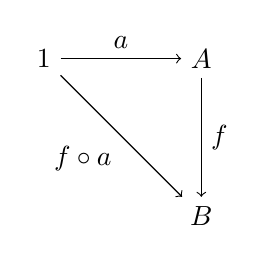
\begin{tikzpicture}[auto]
				\node (a) at (2, 0) {$A$};
				\node (b) at (2, -2) {$B$};
				\node (1) at (0, 0) {$1$};
				\draw[->] (1) to node {$\varDelta a$}(a);
				\draw[->] (1) to node[swap] {$f\circ \varDelta a$}(b);
				\draw[->] (a) to node {$f$}(b);
			\end{tikzpicture}
		\end{center}
  \end{prop}
  \begin{proof}[$\Longrightarrow$]
    \begin{align*}
      f(a) &= b\\
      f(\varDelta a(*)) &= \varDelta b(*)&\text{(定写像の定義)}\\
      f\circ \varDelta a(*)&=\varDelta b(*)&\text{(写像の合成の定義)}\\
      \intertext{$1$の任意の元$*$に対して成り立つから}
      f\circ \varDelta a &=\varDelta b
    \end{align*}
    となる。
  \end{proof}
  \begin{proof}[$\Longleftarrow$]
    上の証明の等式変形を逆に行えば良い。
  \end{proof}

